% !TeX spellcheck = en_US
\documentclass[]{ccs-thesis}
% options:
% [germanthesis] - Thesis is written in German
% [plainunnumbered] - Don't print numbers on plain pages
% [earlydraft] - Settings for quick draft printouts
% [watermark] - Print current time/date at bottom of each page
% [phdthesis] - switch to PhD thesis style
% [twoside] - double sided
% [cutmargins] - text body fills complete page


% Author name. Separate multiple authors with commas.
\author{Philip Frerk}
\birthday{March 31, 1994}
\birthplace{Bielefeld}

% Title of your thesis.
\title{Wireless Protection of Vulnerable Road Users}

% Choose one of the following lines. Feel free to change the word "Informatik" to match your degree program.
%\thesistype{Masterarbeit im Fach Informatik}\thesiscite{Master's Thesis~(Masterarbeit)}
%\thesistype{Bachelorarbeit im Fach Informatik}\thesiscite{Bachelor Thesis~(Bachelorarbeit)}
\thesistype{Seminar Thesis in Computer Science Master's}\thesiscite{Seminar Thesis~(Seminararbeit)}

% List of advisors, separated by commas.
\advisors{Christoph Sommer}

% List of referees, separated by commas.
\referees{Christoph Sommer, Falko Dressler}


% Define abbreviations used in the thesis here.
\acrodef{WSN}{Wireless Sensor Network}
\acrodef{MANET}{Mobile Ad Hoc Network}
\acrodef{ROI}{Region of Interest}{short-indefinite={an}, long-plural-form={Regions of Interest}}
\acrodef{ADAC}{German Automobile Association}{foreign={Allgemeiner Deutscher Automobilclub}}
\acrodef{CANhashing}[CAN]{Content Addressable Network}{extra={when referring to the distributed hash table}}
\acrodef{CANproto}[CAN]{Controller Area Network}{extra={when referring to the bus protocol}}
\acrodef{VRU}{Vulnerable Road User}
\acrodef{GVT}{gefährdeter Verkehrsteilnehmer}
\acrodef{V2PCS}{Vehicle to Pedestrian Communication System}
\acrodef{GDA}{Geographical Destination Area}
\acrodef{POC}{Probability of Collision}
\acrodef{LOS}{Line-of-sight}
\acrodef{NLOS}{Non-line-of-sight}
\acrodef{ITS}{Intelligent Transportation System}

\begin{document}

\pagenumbering{roman}

\maketitle

\TODO{Datum auf englisch machen}

\TODO{erkläruing unterschreiben}

\chapter*{Abstract}
\addcontentsline{toc}{chapter}{Abstract}
\begin{otherlanguage*}{american}

Protecting \acp{VRU} is a very important task as in roughly 50 \% of all traffic accidents \acp{VRU} are involved. \acp{VRU} are pedestrians or drivers of two-wheeled vehicles.
A technology is needed that warns both the \ac{VRU} and the car driver if an accident between them is likely to happen so that they can react accordingly.  This is a challenging task, because the warnings have to be sent in time  and also it has to ensured that no people are warned who are not really affected by the approaching car.
To achieve that goal, Wireless Networking, GPS and Sensor Perception will be used.
Results show that the number of accidents with \acp{VRU} involved can be reduced dramatically.
As the initial results are promising, research in this area is being expanded, especially as there are many further challenges, for example situations with many \acp{VRU} and many cars in dense cities.


\end{otherlanguage*}


\chapter*{Kurzfassung}
\addcontentsline{toc}{chapter}{Kurzfassung}
\begin{otherlanguage*}{ngerman}

Der Schutz von gefährdeten Verkehrsteilnehmern ist eine sehr wichtige Aufgabe, da an rund der Hälfte aller Verkehrsunfälle solche Verkehrsteilnehmer beteiligt sind. Gefährdete Verkehrsteilnehmer sind definiert als Fußgänger oder Fahrer von zweirädigen Fahrzeugen. Es wird eine Technologie benötigt, welche sowohl den gefährdeten Verkehrsteilnehmer als auch den Fahrer eines Autos warnt, wenn es wahrscheinlich ist, dass ein Unfall zwischen ihnen passiert. Das ist eine schwierige Herausforderung, da die Nachrichten schnell genug ausgetauscht werden müssen und auch dafür gesorgt werden muss, dass keine Fußgänger gewarnt werden, die eigentlich nicht in den Unfall verwickelt werden können. Um dies zu ermöglichen, werden Drahtlos-Netzwerke, GPS-Technologie und Computer Vision eingesetzt. Die Ergebnisse zeigen, dass dadurch die Anzahl der Verkehrsunfälle deutlich gesenkt werden kann. Wegen dieser vielversprechenden Resultate wird zukünftig noch mehr Forschungsarbeit in dieses Thema gesteckt werden. Dies ist auch nötig, da die Systeme noch nicht fähig sind, in Situationen mit sehr vielen Fußgängern (bzw. gefährdeten Verkehrsteilnehmern) umzugehen, was aber in dicht besiedelten Städten oft der Fall ist.


\end{otherlanguage*}
\acresetall

\cleardoublepage
\tableofcontents

\cleardoublepage
\pagenumbering{arabic}



\chapter{Introduction}
\label{chap:introduction}

The thesis starts by giving a short motivation for the topic, and then providing an overview about how the work is structured.

\section{Motivation}
\label{sec:motivation}

Within the last century the usage of motorized vehicles has grown rapidly. While this fact brings the great benefit of full mobility, it does not come without its downsides. One of them is the high number of traffic accidents. According to~\cite{v2pcomm} in roughly half of all traffic accidents, \acp{VRU} are involved. Hence, there is huge potential to prevent injuries or even deaths of many people. This thesis will give you an overview of the current state of research in this area. While there are many approaches beyond the discipline of Wireless Networking (e.g. Computer Vision for pedestrian recognition), this thesis will focus mainly on how to prevent traffic accidents by using Wireless Networking Technology. However, the other areas will also be explained briefly since they often work hand in hand with Wireless Networking.

\section{Structure of the Thesis}
\label{sec:structure}

The thesis is structured as follows. Chapter~\ref{chap:v2p} is the main part of the thesis and will show the different ways for protection of \acp{VRU} by using Wireless Networking. In chapters~\ref{sec:special device}, \ref{sec:smartphone}, \ref{sec:beacon}, we will look at different solution which rely solely on Wireless Networking. We will then see why such systems are often not satisfying, and in chapter \ref{sec:fusion} we will take a look at an approach which combines Wireless Networking and Sensor Perception in order to improve the performance and precision.

Finally, in chapter~\ref{chap:conclusion} all the approaches will be summarized and also we will see what future tasks are still left in this area to make it usable in the real world.


\chapter{Protecting Vulnerable Road Users}
\label{chap:v2p}

The basic idea behind \acp{V2PCS} is that a driving vehicle (most often a car) and a \ac{VRU} (most often a pedestrian) exchange messages over a wireless network in order tell each other their positions. By doing that, accidents between them can be prevented because both the car driver and the pedestrian can react to the received messages.

There are several approaches to implements such a system and they will be discovered in this chapter.

\section{Special Device as Warning Unit}\label{sec:special device}

First, we will look at such communication systems which use a special device for the \ac{VRU} in order to send his messages. In \cite{v2pprotection} and \cite{watchover} such systems have been proposed. \TODO{watchover genauer}

The device from \cite{v2pprotection} can be seen in the bottom of figure~\ref{fig:device}. In the top of figure~\ref{fig:device} you can see the warning unit that will be installed in the car.

\begin{figure}[h]
	\centering
	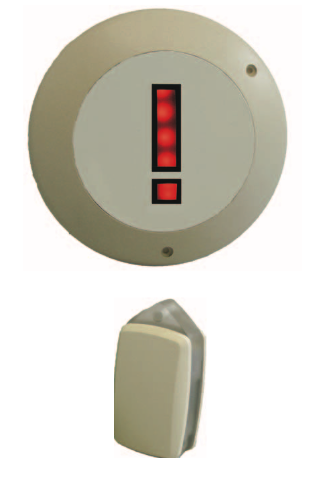
\includegraphics[width=0.3\textwidth]{figures/1_device}
	\caption{The Warning Unit for Cars and the Warning Device for Pedestrians from \cite{v2pprotection}}%
	\label{fig:device}%
\end{figure}

The task of the device for the pedestrian is to periodically send \enquote{Hello}-Messages including the pedestrian's position so that the warning unit in the car can receive those messages and detect a probably dangerous situation. Then the warning unit sets itself into a warning status (which can be seen in figure~\ref{fig:device}).

It is very important that the car driver does not get too many warning messages because otherwise he would loose sensibility for the warning. Therefore, a key issue is to ensure that only warning are created if the distance between car and pedestrian decreases gradually.

Figure~\ref{fig:chart1} shows the alerting probability on the y-axis and the distance between the person and the car on the x-axis. The alerting probability decreases as the distance increases, as expected. The red parts of the bars represent the amount of meaningful warnings, which are roughly half of all warnings, because in this test scenario only one pedestrian is present. That ratio is not satisfying, but this is only because of the low number of pedestrians.

In figure~\ref{fig:chart2} you see the same statistics, but for a scenario with 10 pedestrians. Here the ratio is almost 100\%, due to the higher number of pedestrians which makes it way more likely that a warning is meaningful, and such a scenario will be more likely in real world conditions, for example in cities.

\begin{figure}[h]
	\centering
	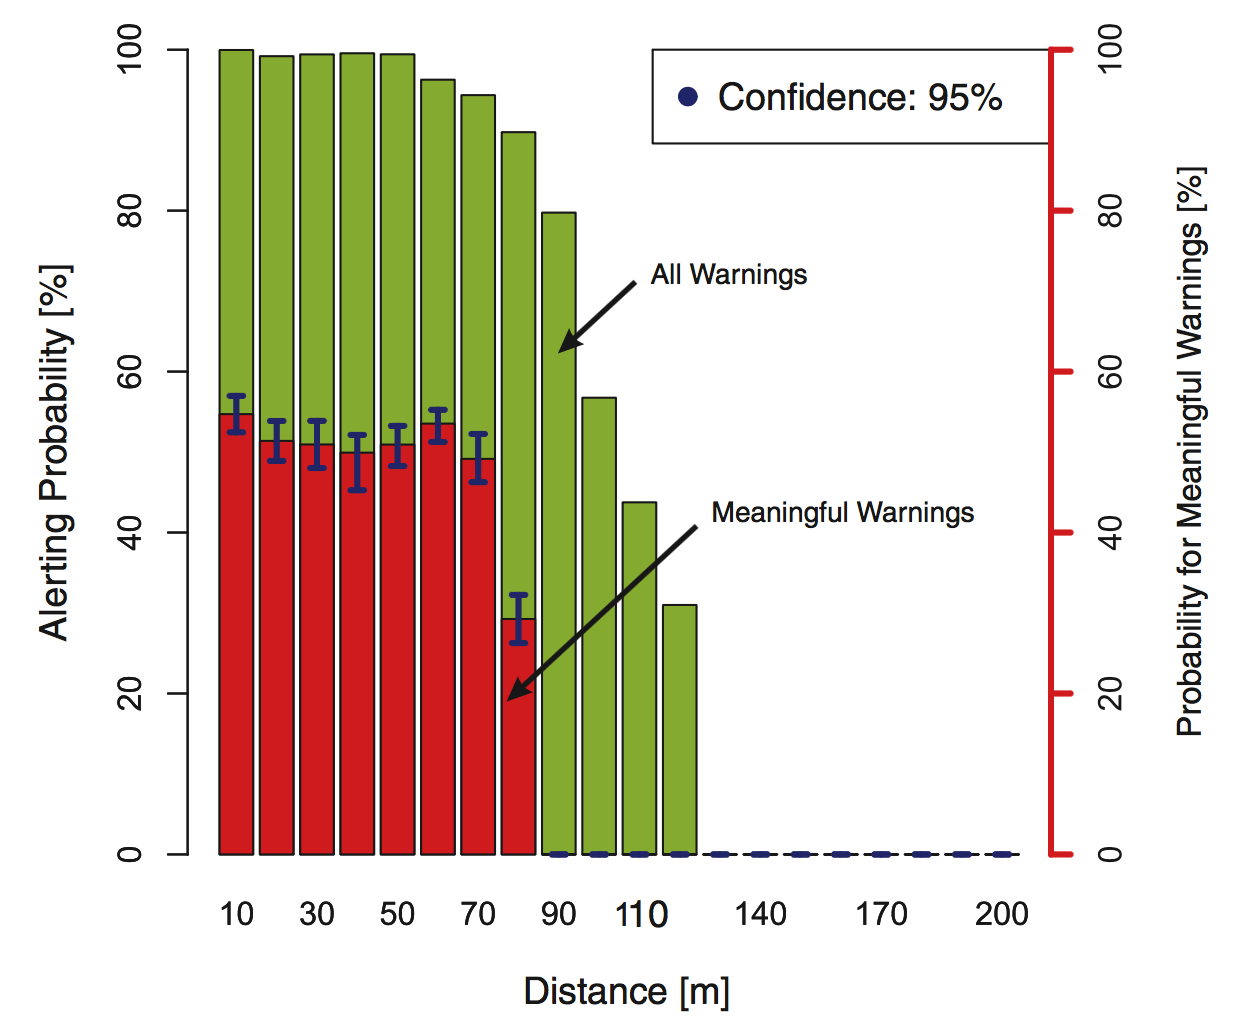
\includegraphics[width=0.8\textwidth]{figures/2_chart}
	\caption{Warning statistics in a test scenario with one pedestrian from \cite{v2pprotection}}%
	\label{fig:chart1}%
\end{figure}

\begin{figure}[h]
	\centering
	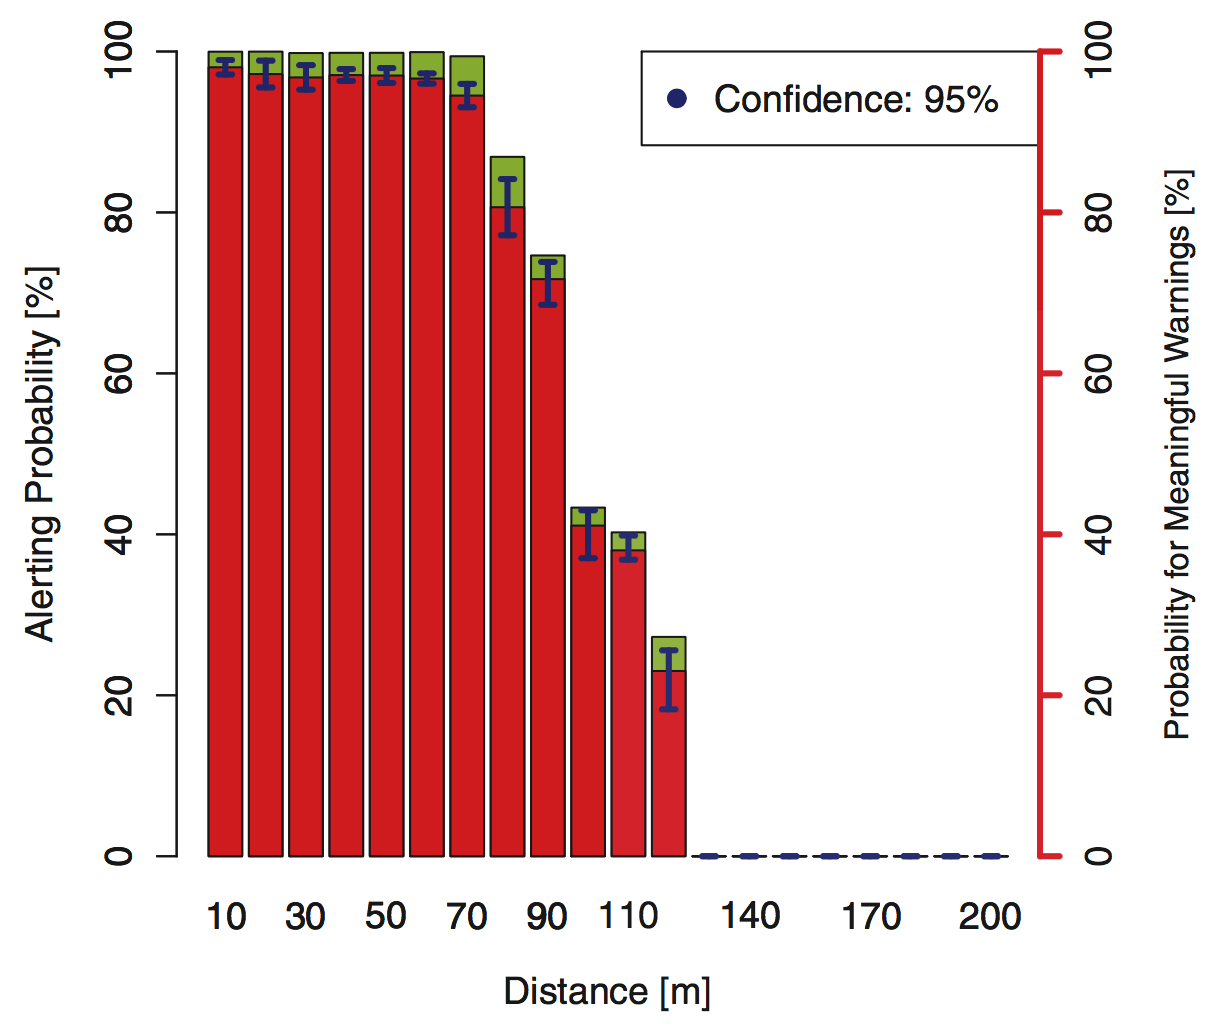
\includegraphics[width=0.8\textwidth]{figures/3_chart}
	\caption{Warning statistics in a test scenario with 10 pedestrians from \cite{v2pprotection}}%
	\label{fig:chart2}%
\end{figure}


\section{Smart Phones as Warning Devices}\label{sec:smartphone}

In \cite{v2pcomm}, another approach has been developed which is based on the same idea as \cite{v2pprotection}, but it is more detailed. Moreover, it has the great benefit that no additional device for the \ac{VRU} is needed because in this system a smart phone or tablet will be used as the warning device for the pedestrians.

The approach is more detailed, because it formulates precise requirements that an implementation of a \ac{V2PCS} should have in order to be able to work in reality. The  requirements basically boil down to the following: One has to calculate the distance between the car and the pedestrian at which the warning messages are to be delivered. In section~\ref{sec:special device} we have already seen that this distance should not be too big, because otherwise too many meaningless warning would be received. But accordingly, the distance must not be too small, because the pedestrian and the car driver must have enough time to react to the messages.

To calculate this distance, the authors of \cite{v2pcomm} have taken into consideration many parameters, e.g. the velocity of the car, the reaction time of the pedestrian, the expected positioning error of GPS (which is approximately 10m), the expected packet transmission time of Wi-Fi and so on. As an example, we take a look at equation~\ref{equi:minDistance} where the lower bound $d_{min}$ of the distance is written down.
\begin{align}
d_{min}=v \times (t_p+t_r+t_{tx})+gnss_{err_{car}}+gnss_{err_{ped}}\label{equi:minDistance}
\end{align}
Here $v$ is the car's velocity. Moreover, $t_p$ is the time for Perception of the pedestrian, $t_r$ is the reaction time of the pedestrian, and $t_{tx}$ is the packet transmission delay. $gnss_{err_{car}}$ and $gnss_{err_{ped}}$ are the positioning errors of the car and the pedestrian, respectively.

For simplification, we will not look in every detail of this calculation as it is very detailed. But in principle it is crucial to compute a lower and upper bound for the distance at which the warning messages should be sent. Because you can then check whether your system always fulfills these bounds which the system from \cite{v2pcomm} does.

Finally, the distance calculated is 39.5, 52.3, and 72.0 m, when the velocity of the car is 30, 50, 80 km/h, respectively. \cite{v2pcomm}
\\\\
Another important concept in this context of when to send warning messages is the so called \ac{GDA}. You can understand the concept by considering figure~\ref{fig:gda}. In (a) a car is approaching to pedestrians, P1 and P2. As the car is yet far away from P1 and P2 it is possible that both P1 and P2 could be involved in an accident with the car, therefore both of them are in the \ac{GDA} (green area).

In (b) the car has already come nearer to P1 and P2 and is currently turning left. Due to that fact, it is no longer possible for the car to approach the position of P2. So, P2 is no longer in the \ac{GDA} of the car and P2 will not receive a warning message, only P2 will get one.

\begin{figure}[h]
	\centering
	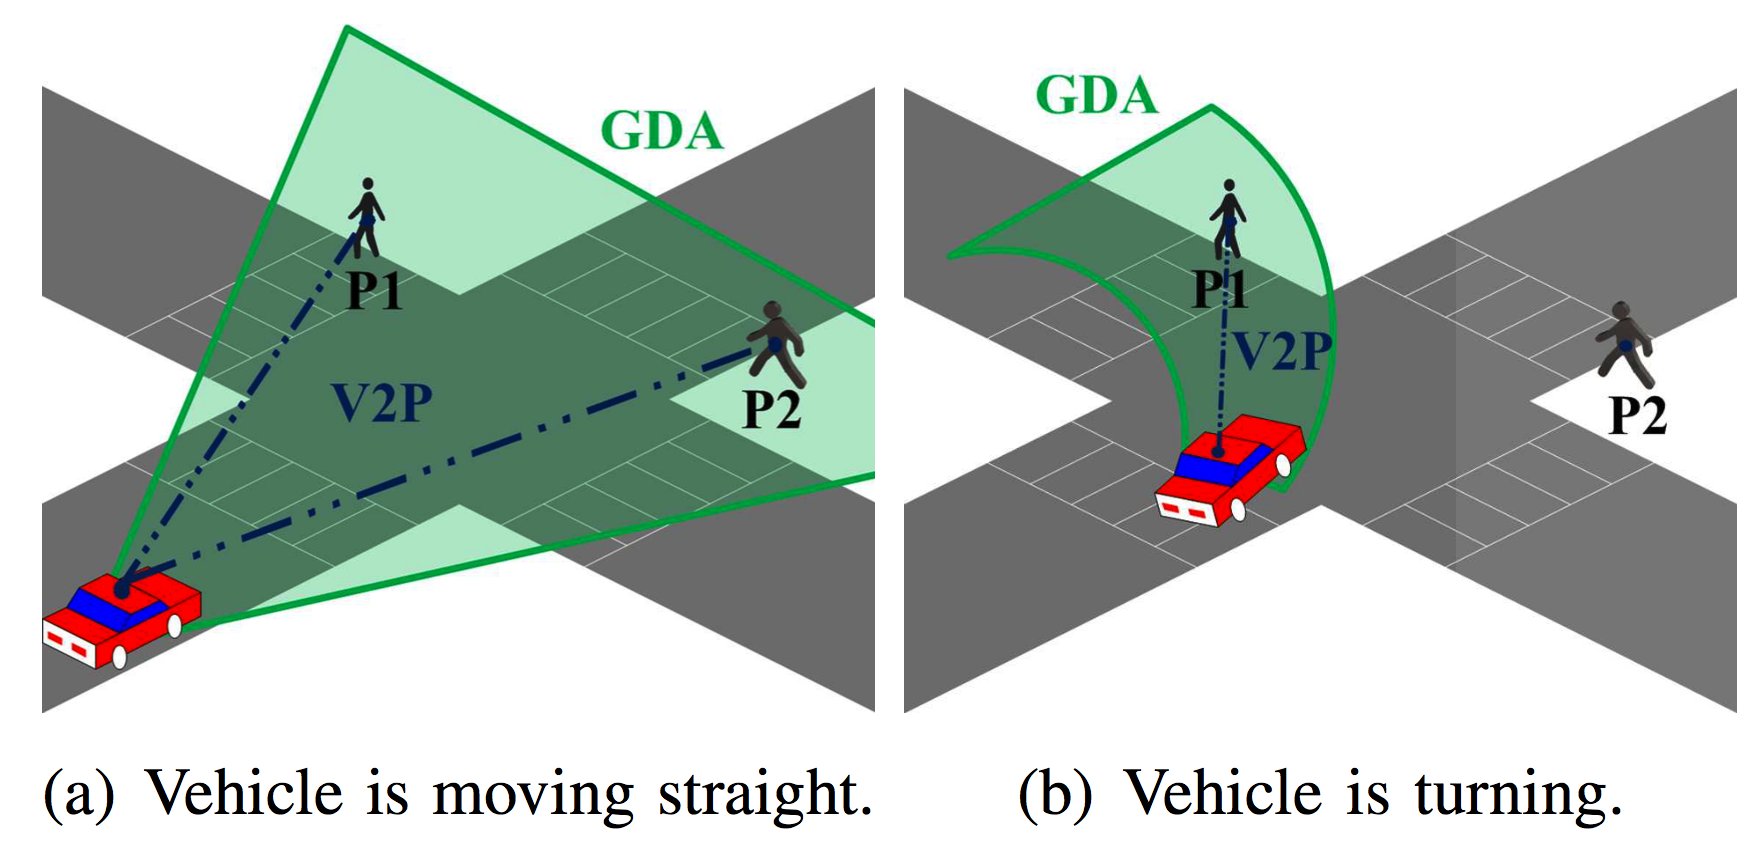
\includegraphics[width=0.8\textwidth]{figures/5_gda}
	\caption{The Geographical Destination Area of a moving car at two different points in time, from \cite{v2pcomm}}%
	\label{fig:gda}%
\end{figure}

The \ac{GDA} of a car will be computed periodically and this makes sure that even less meaningless warning messages will be sent. The \ac{GDA} can be computed by taking several parameters of the car (e.g. the yaw rate, speed, etc.) into account.

\section{Faster WiFi Message Exchange by using Beacon Stuffing}\label{sec:beacon}

The principle from chapter~\ref{sec:smartphone} has one disadvantage that has not yet been emphasized.
Typically, when two devices want to communicate with each other over WiFi, they have to establish a WiFi connection first. This process usually takes a few milliseconds which can be crucial in such a dynamic situation. But there is an approach from the authors of \cite{beacon} to avoid that connection establishing phase by using WiFi Beacon Stuffing. Beacons are usually used in order to propagate the existence of a WiFi network. They are broadcasted periodically by the WiFi access point and contain information about the network (e.g. the SSID).

In \cite{beacon} the SSID field is replaced by a so called WiFi Honk Information Packet, which includes information about the moving car, namely the latitude, longitude, speed, and direction. \acp{VRU} or other cars then receive this information and compute the likelihood of an accident.

Figure~\ref{fig:beacon} shows the results of~\cite{beacon} compared to WiFi without Beacon Stuffing. Sub figure (a) shows that pedestrians have a little more time to react, but obviously if the velocity of the car comes close to 100 mph there is almost no time to react. Sub figure (b) shows the \ac{POC} after receiving an alert, depending on the car's speed, on which Beacon Stuffing has a decisive impact. \ac{POC} is defined in equation~\ref{equ:poc}.

\begin{align}\label{equ:poc}
\text{POC}=\dfrac{\text{Required Time To Stop}}{\text{Time to Recognize Alert}+\text{Time Available to Stop }}
\end{align}

POC is much smaller when using Beacon Stuffing, because \enquote{Time to Recognize Alert} and \enquote{Time Available to Stop} become greater. Due to the higher \ac{POC}, warning messages can be sent more aggressively in the WiFi Honk Mode.

The Beacon Stuffing approach is a useful technique which can be added to \acp{V2PCS} to enhance the packet transmission time.

\begin{figure}[h]
	\centering
	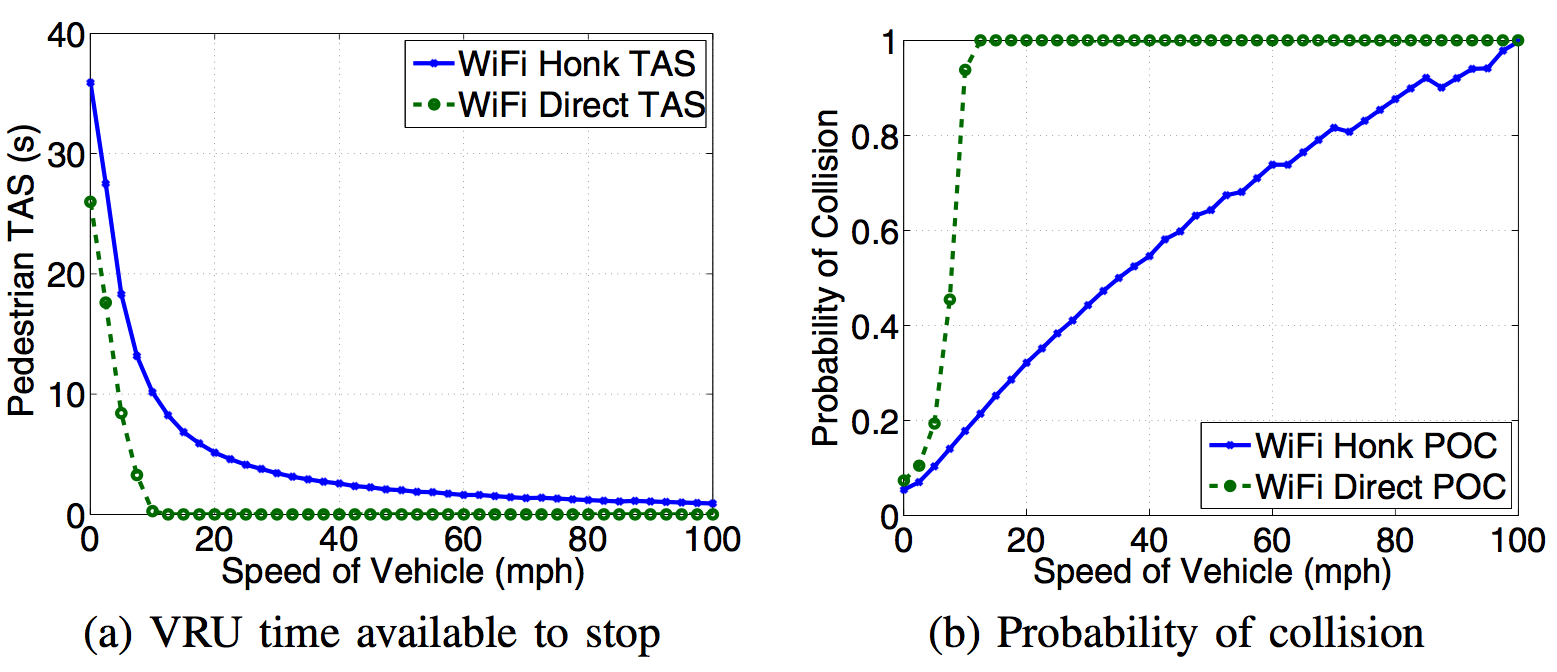
\includegraphics[width=1\textwidth]{figures/6_beacon}
	\caption{Evaluation of Beacon Stuffing, from \cite{beacon}.}%
	\label{fig:beacon}%
\end{figure}

\section{Fusion of Perception and V2P Communication}\label{sec:fusion}

Apart from the discipline of Wireless Networking there is another approach for detecting \acp{VRU}. Nowadays, cars are equipped with sensors which are supposed to detect objects in the environment. In \cite{survey} the different types of sensors are presented. First, cameras are used as sensors, when pictures are taken, the interesting information has to extracted from the picture. In~\cite{2010perception}, the authors explain how the extraction works. In the first step, the so called noise has to be removed from the picture, in particular the background. In the second step, the different objects in the picture have to be classified, e.g. a tree is not as important as a pedestrian. This process is done by Machine Learning Algorithms and it is difficult due to the fact that humans look quite differently, as the can have different heights, can carry around other objects, or ride on bicycles. 

Because of the complexity of the classification step, other types of sensors are presented in~\cite{survey}. Thermal sensors can be used which detect humans by their body heat. Therefore, they can locate humans very precisely and a classification step is not necessary. But in hot day conditions, they are not reliable, because the heat difference becomes smaller.

Nowadays, lasers are used most often as they are very precise and work in all weather conditions. Some years ago lasers were very expensive, but after the development in the last years they have become affordable.

The biggest disadvantage of using sensors for pedestrian detection is that they are not able to work when the pedestrian is occluded by an obstacle. So, it is not satisfying to only use Sensor Perception for protecting \acp{VRU}. But in fact, Sensor Perception has also some advantages in comparison to \acp{V2PCS}. 

That is demonstrated by figure~\ref{fig:fusion} where in sub figure~\ref{fig:fusion} (a) the Perception System determines the position of the pedestrian more precisely. The blue triangle is the position transmitted by WiFi Communication (by using GPS), and the red circle is the position calculated by the Perception System. The Perception System works better here, because this is a \ac{LOS} situation which means that the pedestrian is not occluded by any obstacle. The Perception System is capable of determining positions very precisely whereas GPS can always have a small positioning error, as mentioned earlier.

In sub figure~\ref{fig:fusion} (b) the condition is different, there we are confronted with a \ac{NLOS} situation. So, the pedestrian is not detected by the Perception System, because lasers or cameras obviously cannot look through obstacles. But the \ac{V2PCS} still detects the pedestrian (blue triangle).

\begin{figure}[h]
	\centering
	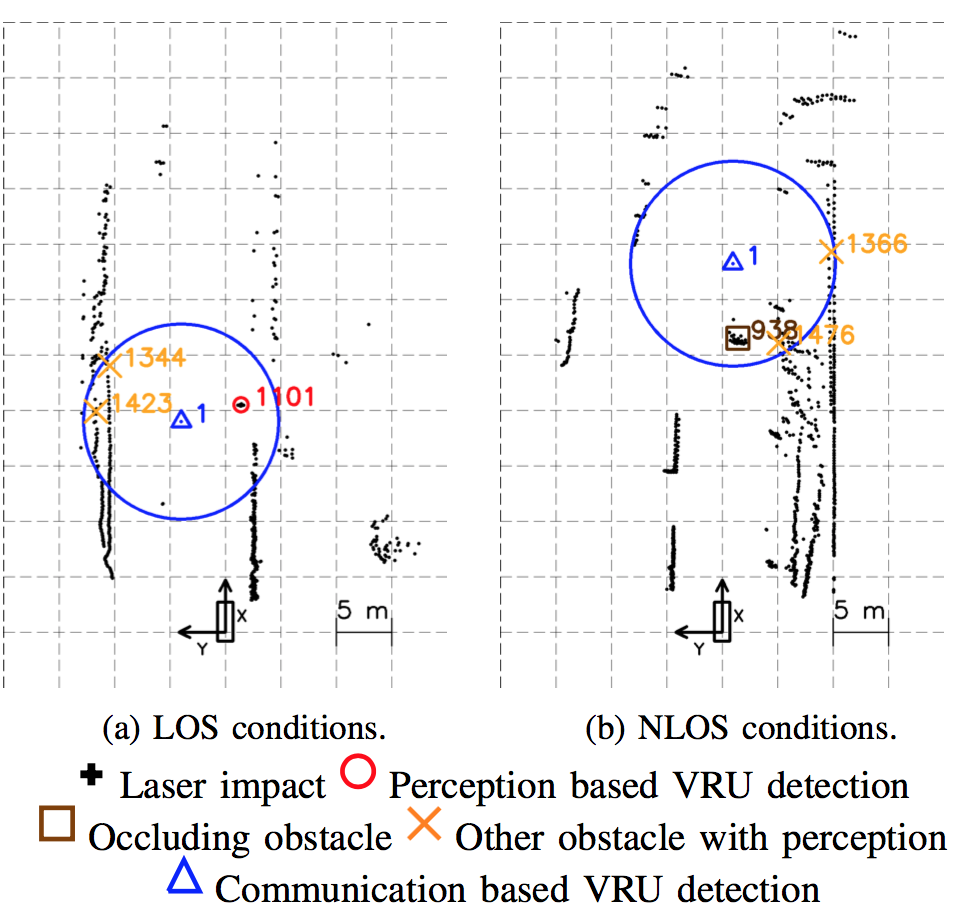
\includegraphics[width=0.9\textwidth]{figures/7_fusion}
	\caption{Two different scenarios for \ac{VRU} detection, from \cite{2016fusion}\\ In (a) Perception works better (due to \ac{LOS} conditions) and in (b) WiFi communication works better (due to \ac{NLOS} conditions).}%
	\label{fig:fusion}%
\end{figure}

After seeing the advantages and disadvantages of both Perception Systems and \acp{V2PCS} the big task is now the fusion of data generated by the two systems. Since this process is quite complicated only the core idea will be explained here.

The objective of the fusion is to determine whether a communicating \ac{VRU} is visible or hidden by some obstacle. In order to understand that, we take a look at sub figure~\ref{fig:fusion} (a) again. The big blue cycle represents the area in which the pedestrian can be located, considering the GPS positioning error from the transmitted position of the pedestrian via the \ac{V2PCS}. In (a) the pedestrian is visible, so the system could associate him with some of the objects in the blue area. But obviously, it should associate him with the correct object (the pedestrian himself). This can be done by receiving many tracks of the \ac{V2PCS}, which will all be a little different due to the GPS positioning error. By looking at the set of those different locations, you can see that they will settle around a particular object detected by the Perception System and so the combined system can select the correct object and take the location computed by the Perception System as it is more precise.

In contrast, in sub figure~\ref{fig:fusion} (b) the pedestrian is not visible. So, the Perception System will only detect other objects in the blue area. Again, by looking at the several tracks from the \ac{V2PCS}, you realize that they will not settle around any of the objects detected by the Perception System. Therefore, you can conclude that the Perception System has not detected the pedestrian and rely solely on the data of the \ac{V2PCS} (GPS position).
\\\\
The results from \cite{2016fusion} show that the combined system benefits from the advantages from both the \ac{V2PCS} and the Perception System. In \ac{LOS} conditions, the system can locate the pedestrian more precisely because of the very precise data from the Perception System. As the distance between the car and the pedestrian increases, the Perception becomes useless, and only the data from the \ac{V2PCS} can be used. The same holds for \ac{NLOS} conditions. Moreover, the combined has yet not been tested for situations with many communicating cars and pedestrians which will strain the system more. Nevertheless, the fusion approach is a very useful and promising technique for \ac{VRU} protection.

\section{Wireless Protection of Motorbikes}\label{sec:motorbikes}

We will now look into a different topic, which is protecting drivers of motorbikes by using Wireless Networking. Yet we have focused mainly on pedestrians as \acp{VRU}, but motorbike drivers are \acp{VRU} as well, and due to the high popularity of motorbikes this area is also very important. 

There are already approaches for so called \acp{ITS}, for example in~\cite{its}. There, Wireless Sensor Networks are used in order to exchange information between cars.  Those systems are also designed to enhance efficiency on the road, but of course also in order to provide more safety. Therefore, the cars will exchange messages including the typical parameters like speed, direction etc.

But those \acp{ITS} typically do not focus particularly on motorbikes, as the requirements for motorbikes are partly different to the ones for cars. In~\cite{bikes} such an integration of motorbikes into existing \acp{ITS} has been proposed.

One of the special requirements for motorbikes is that the communication system has to consume less energy than in cars. Therefore, the hardware from~\cite{bikes} is battery-powered. Also the human interface on a motorbike cannot be as rich as in car. Therefore, LEDs and a buzzer can be used.

The system works as follows. It receives the several messages from other vehicles including information like speed, direction etc. It then maintains a database of vehicles nearby and computes which other cars can possibly be involved in an accidents with the own motorbike by taking into account the own speed, direction etc. (analogously to a \ac{V2PCS} as we have seen before). If it detects a dangerous situation the driver will be warned by the blinking LEDs and the buzzer.

Of course, the systems also broadcasts its data to other vehicles over WiFi in order to inform them.

Apart from that, the system is also capable of running in cars, and in that case informs the driver about nearby motorbikes. In contrast, when running in a motorbike, the system focuses on warning the driver about nearby cars as they are a bigger threat for the motorbike driver.

A future task will be to make the system runnable in 4G networks as well in order to improve the performance.

\chapter{Conclusion}
\label{chap:conclusion}


This thesis gave an overview of the current state of research in the area of protecting \acp{VRU} by mainly using Wireless Networking. That topic is of high interest because many accidents happen between vehicles and \acp{VRU}, so a large number of accidents could be prevented.

This protection basically works by exchanging messages between \acp{VRU} and cars over a wireless channel and then calculating the likeliness of an accident between the two. We have also seen that a \ac{V2PCS} as stand alone are not sufficient, mostly due to the imprecision of GPS. Therefore, sensor Perception will be used in addition, as those sensors are generally more precise than GPS. The fusion of those two types of \ac{VRU}-detection can then benefit from the advantages of both WiFi and Perception, whereby the disadvantages (imprecision of GPS and low range of Perception) can be eliminated.

Apart from that, we have also considered motorbikes as another class of \acp{VRU}. The main goal is to integrate motorbikes in \ac{ITS}-systems that are already under development, but mostly for cars. This is challenging because of the special requirements that motorbikes will yield (e.g. less energy consumption, more compact human interface etc.).

In general, you can state that there two different approaches for future research, either focusing on the fusion of V2P Communication and Perception, or concentrating on a technology more precise than GPS and then only using V2P Communication. Those technologies are currently under development, like the one in~\cite{doppler}, where GPS is extended and the accuracy is improved by up to 48\%. 

The future work will show which way will lead to better results.



\cleardoublepage

\listofabbreviations
\clearpage

\listoffigures
\clearpage

\TODO{bib wieder anzeigen}
%\printbibliography


\end{document}